% !TEX program = xelatex

\documentclass[aspectratio=169]{beamer}

\usepackage{xltxtra} 
\usepackage{fontspec}
\usepackage{listings}
\usepackage{color}
\usepackage{amsmath}
\usepackage{smartdiagram}
\usepackage{graphicx}
\usepackage{multicol}
\usepackage{tikz}
\usepackage{listings}
\usepackage{multicol}


\usetheme{metropolis}
\XeTeXlinebreaklocale "th_TH"
\defaultfontfeatures{Mapping=tex-text,Scale=MatchLowercase}

\definecolor{codegreen}{rgb}{0,0.6,0}
\definecolor{codegray}{rgb}{0.5,0.5,0.5}
\definecolor{codepurple}{rgb}{0.58,0,0.82}
\definecolor{backcolour}{rgb}{0.95,0.95,0.92}

\lstdefinestyle{defaultstyle}{
    backgroundcolor=\color{backcolour},   
    commentstyle=\color{codegreen},
    keywordstyle=\color{magenta},
    numberstyle=\tiny\color{codegray},
    stringstyle=\color{codepurple},
    basicstyle=\footnotesize,
    breakatwhitespace=false,         
    breaklines=true,                 
    captionpos=b,                    
    keepspaces=true,                 
    numbers=left,                    
    numbersep=5pt,                  
    showspaces=false,                
    showstringspaces=false,
    showtabs=false,                  
    showlines=false,
    tabsize=4
}

\lstset{
	escapeinside=||
}

\title{Python for Data Science}
\author{Sirakorn Lamyai}
\institute{Student, Kasetsart U.}

\begin{document}

\maketitle

\begin{frame}
    \frametitle{About me}
    \begin{columns}
        \column{0.3\textwidth}
            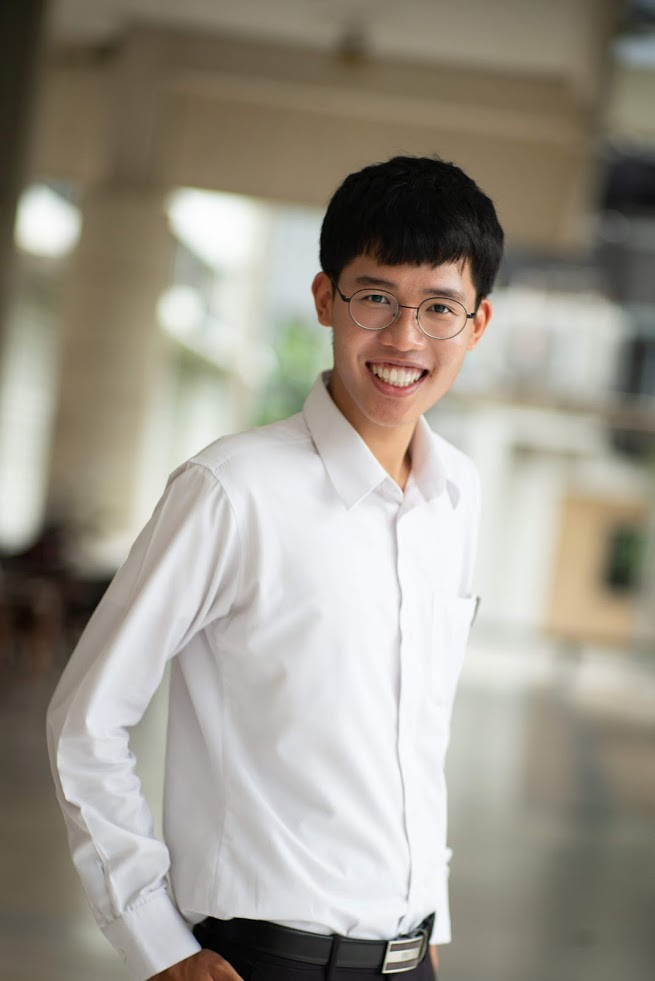
\includegraphics[height=0.8\textheight]{images/sirakorn-1.jpeg}
        \column{0.7\textwidth}
            {\large \textbf{Sirakorn Lamyai}}
            \begin{itemize}
                \item DAKDL Laboratory, Kasetsart University
                \item Research Assistant Intern, 2019, Vidyasirimedhi Institute of Science and Technology
                \item Research Assistant Intern, 2018, Vidyasirimedhi Institute of Science and Technology
                \item Love drinking tea
                \item Knows a little about Python
            \end{itemize}
    \end{columns}
\end{frame}

\begin{frame}
    \frametitle{I know a little about Python}
    When I say I know \textit{a little} about Python\dots
    \begin{itemize}
        \item I think there's some better methods than I'm using
        \item I think I do sometimes make mistakes
        \item There are tons of people who know things much more than me
        \item I think there's much more for me to learn!
    \end{itemize}
\end{frame}

\begin{frame}
    \frametitle{Prerequisite}
    A basic Python knowledge will do!
\end{frame}

\begin{frame}
    \frametitle{Your expectations from this talk}
\end{frame}

\begin{frame}
	\frametitle{Outline}
    \tableofcontents
\end{frame}

\section{Data Science}

\begin{frame}
    \frametitle{The Data Science Process: OSEMNI}
    \begin{itemize}
        \item \textbf{Obtain} data from relevent sources
        \item \textbf{Scrub}, sanitise, and clean the data into machine-understandable formats
        \item \textbf{Explore} significant and meaningful patterns with statistical methods
        \item \textbf{Model} construction for prediction and forecast
        \item \textbf{iNterpret} and use the results obtained
        \item \textbf{Interate} and rethink about your outputs
    \end{itemize}
\end{frame}

\begin{frame}
    \frametitle{Why data?}
    \centering
    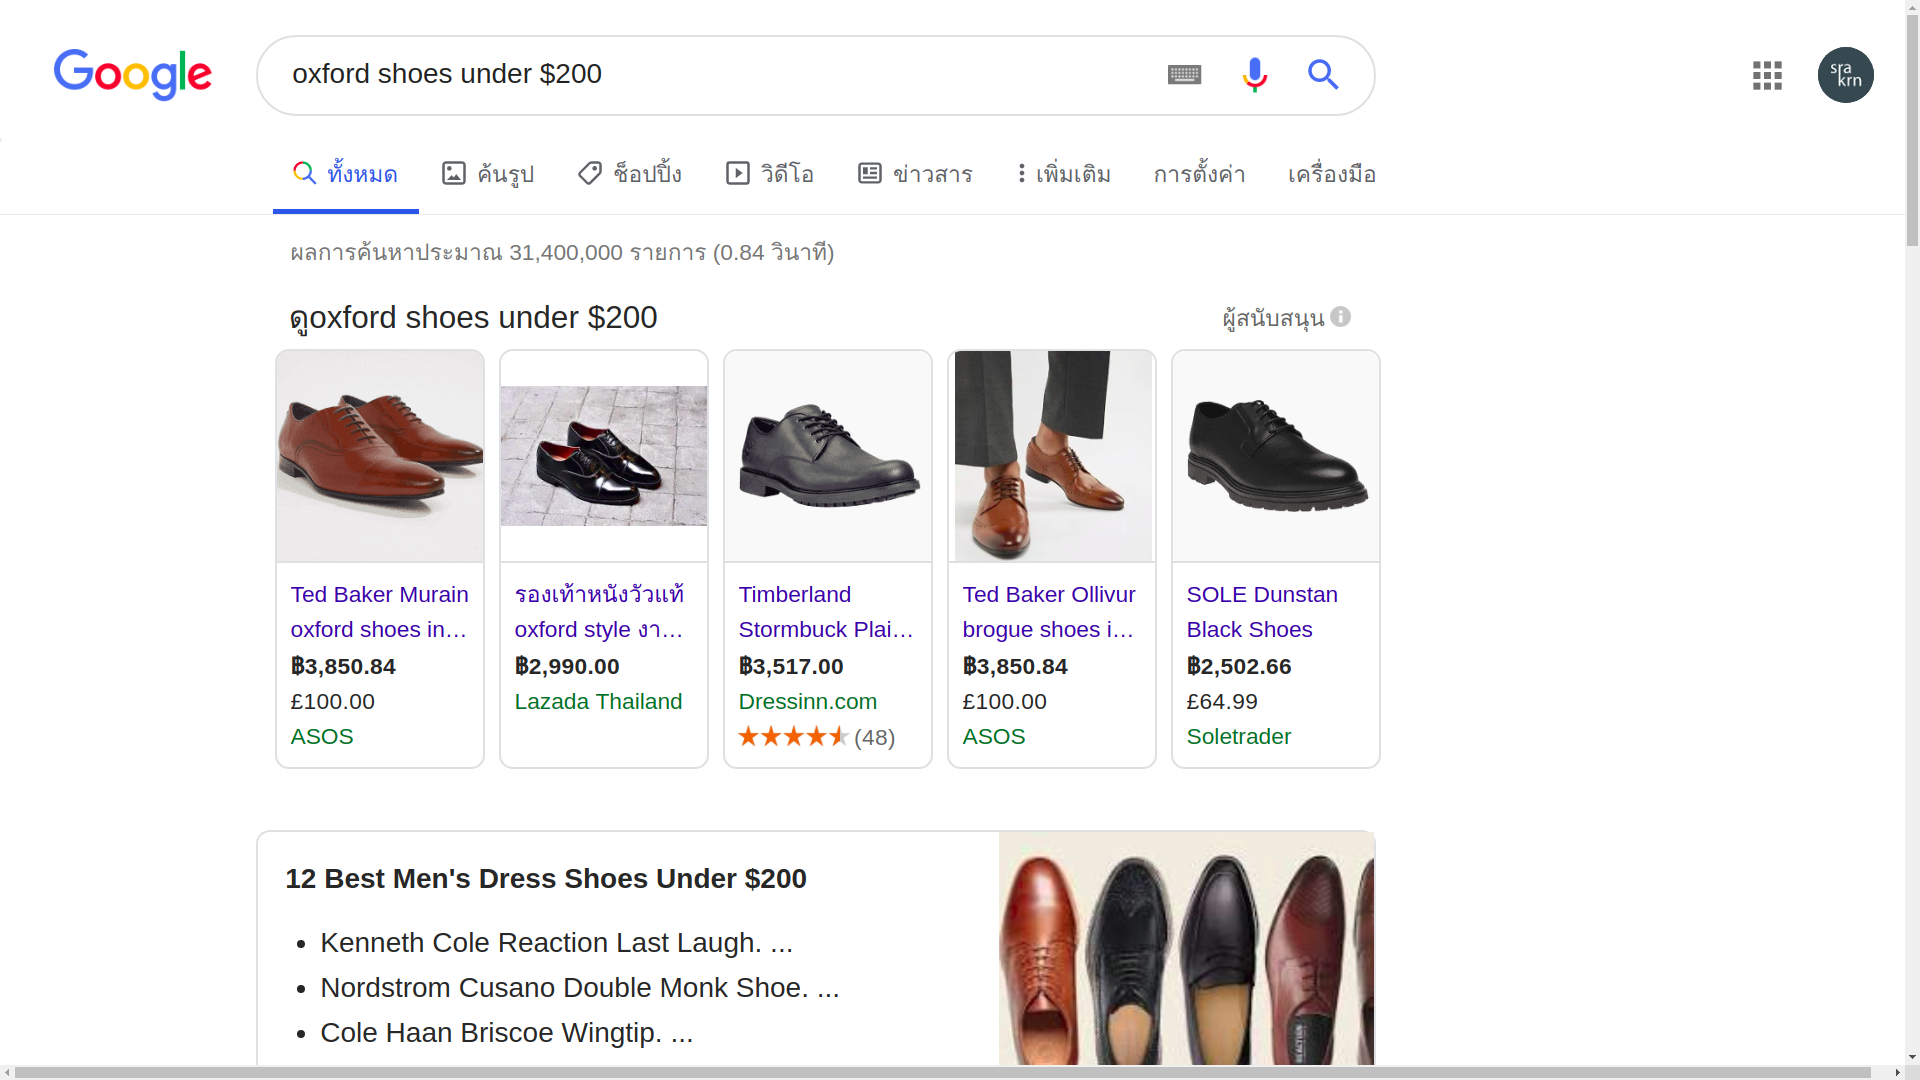
\includegraphics[width=0.8\textwidth]{images/leather-shoes-google.png}
\end{frame}

\begin{frame}
    \frametitle{Why data?}
    \centering
    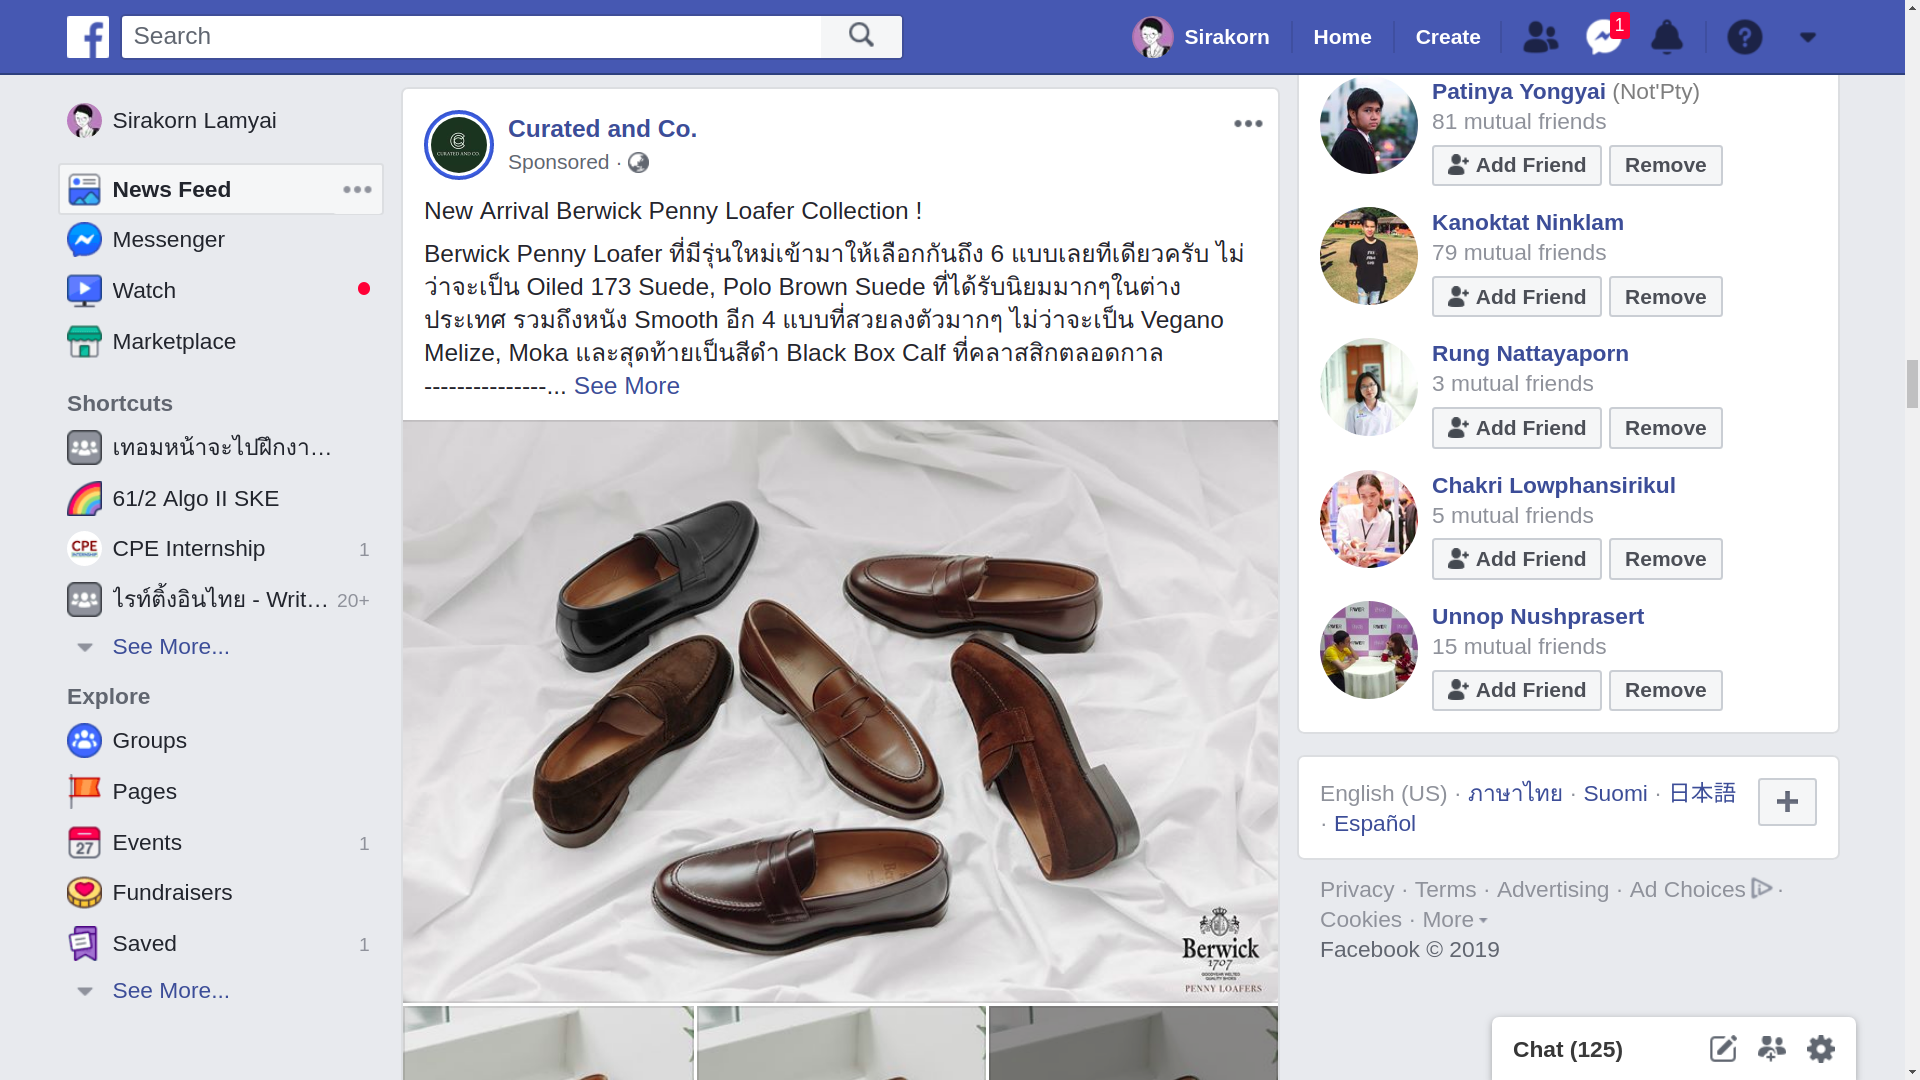
\includegraphics[width=0.8\textwidth]{images/facebook-ads.png}
\end{frame}

\begin{frame}
    \frametitle{Why data?}
    \centering
    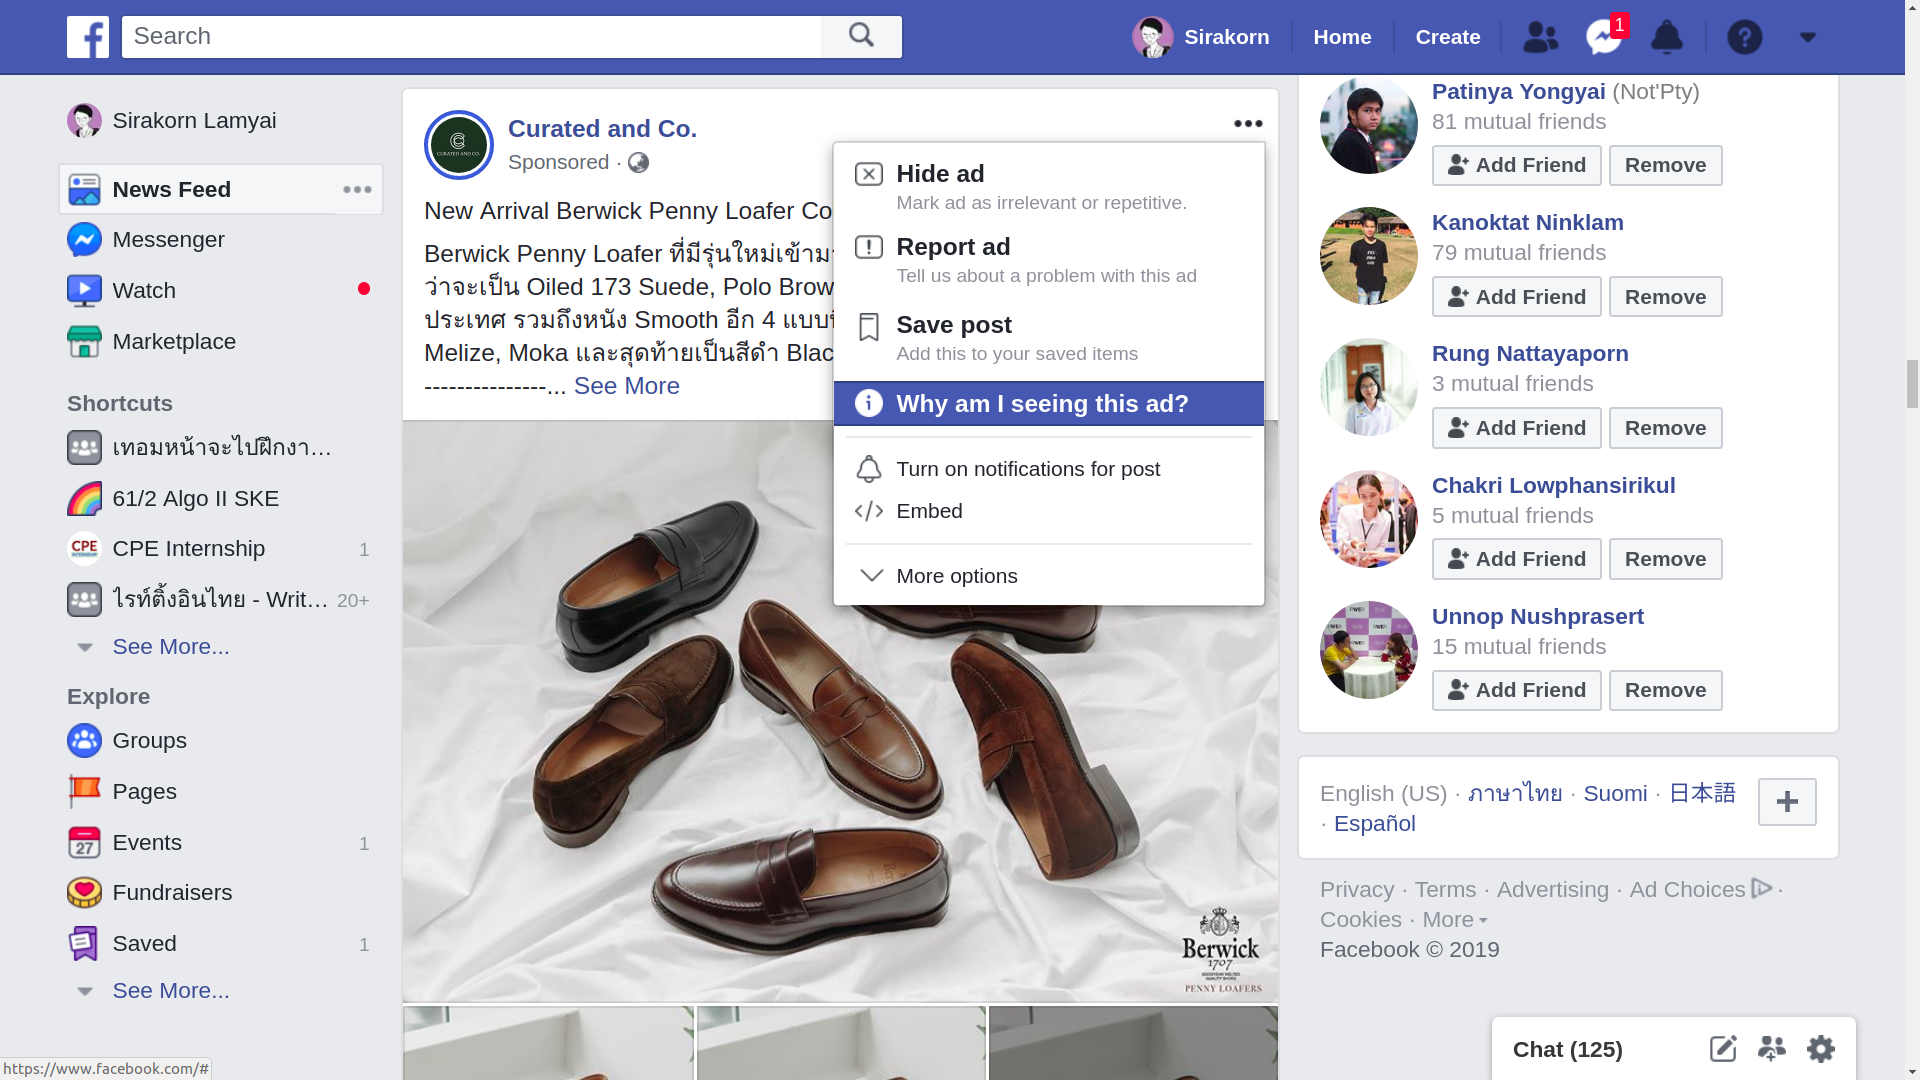
\includegraphics[width=0.8\textwidth]{images/facebook-ads-why-am-i-seeing.png}
\end{frame}

\begin{frame}
    \frametitle{Why data?}
    \centering
    % Zoom 175% on Chrome on Linux to replicate screenshot at this scale
    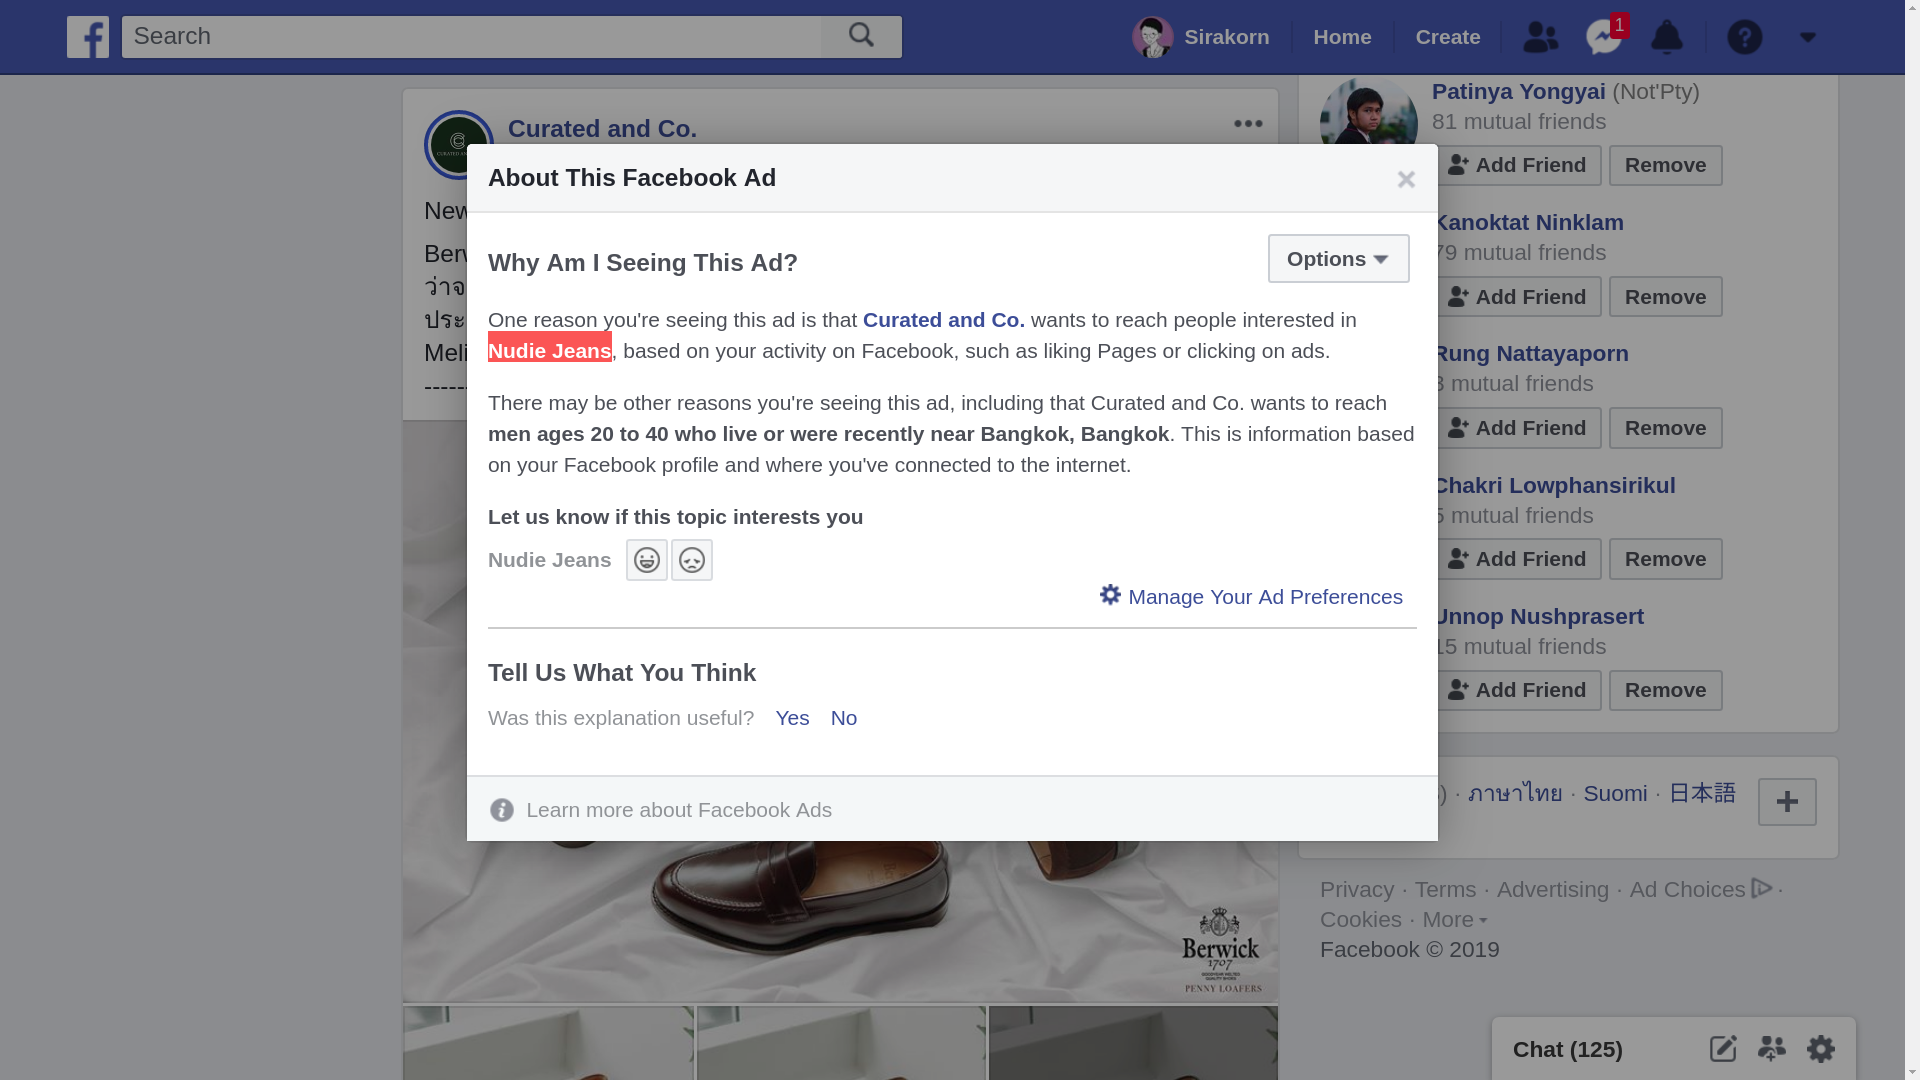
\includegraphics[width=0.8\textwidth]{images/facebook-ads-details.png}
\end{frame}

\begin{frame}
    \frametitle{Why data?}
    \centering
    \Huge Data is the new oil
\end{frame}

\begin{frame}
    \frametitle{Tools for data analysis}
    \begin{columns}[t]
        \column{0.5\textwidth}
            {\large \textbf{With GUIs}}
            \begin{itemize}
                \item Spreadsheets
                \begin{itemize}
                    \item Excel
                    \item Google Spreadsheets
                    \item Lotus 1-2-3
                \end{itemize}
                \item Modelling and Visualisation
                \begin{itemize}
                    \item RapidMiner Studio
                    \item Weka
                    \item Tableau
                \end{itemize}
            \end{itemize}
        \column{0.5\textwidth}
            {\large \textbf{As programming languages}}
            \begin{itemize}
                \item For data insights
                \begin{itemize}
                    \item R
                    \item Python
                \end{itemize}
                \item For data retrieval
                \begin{itemize}
                    \item SQL
                \end{itemize}
            \end{itemize}
    \end{columns}
\end{frame}

\section{Python}

\begin{frame}
    \frametitle{Python}
    \centering
    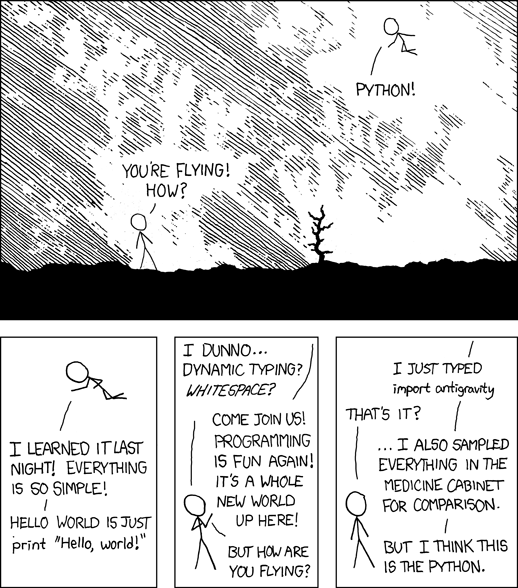
\includegraphics[scale=0.3]{images/xkcd-python.png}

    {\small Courtesy: xkcd (\url{https://xkcd.com/353/})}
\end{frame}

\begin{frame}
    \frametitle{I \textit{loved} Python...}
    \begin{itemize}
        \item Read it, understand it
        \item Multiparadigm
        \item Batteris included
        \item Lots of great, great libraries!
    \end{itemize}
\end{frame}

\begin{frame}
    \frametitle{...yet sometimes I still feels bad with it.}
    \centering
    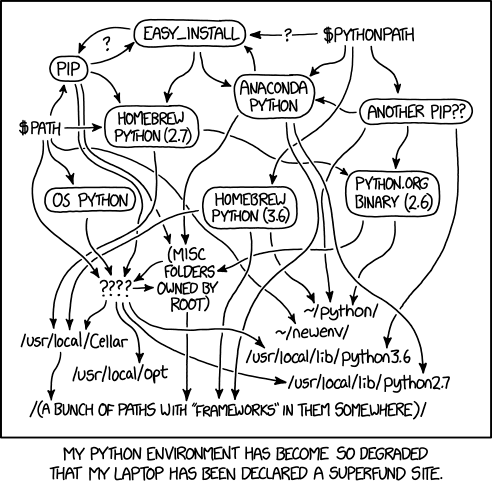
\includegraphics[scale=0.35]{images/xkcd-python-env.png}

    {\small Courtesy: xkcd (\url{https://xkcd.com/1987/})}
\end{frame}

\subsection{Python environments}

\begin{frame}[fragile]
    \frametitle{Environments 101: \texttt{\$PATH}}
    \begin{lstlisting}[style=defaultstyle, language=bash]
$ echo $PATH
/home/srakrn/.pyenv/plugins/pyenv-virtualenv/shims:/home/srakrn/.pyenv/shims:/home/srakrn/.pyenv/bin:/home/srakrn/.local/bin:/usr/local/bin:/usr/local/sbin:/home/srakrn/.local/bin:/usr/sbin:/usr/bin:/sbin:/bin:/usr/games:/usr/local/games:/snap/bin\end{lstlisting}
\end{frame}

\begin{frame}[fragile]
    \frametitle{Environments 101: \texttt{\$PATH}}
    \begin{multicols}{2}
        \begin{itemize}[<+(1)->]
            \item \texttt{/home/srakrn/.pyenv/plugins/pyenv-virtualenv/shims}
            \item \texttt{/home/srakrn/.pyenv/shims}
            \item \texttt{/home/srakrn/.pyenv/bin}
            \item \texttt{/home/srakrn/.local/bin:/usr/local/bin}
            \item \texttt{/usr/local/sbin}
            \item \texttt{/home/srakrn/.local/bin}
            \item \texttt{/usr/sbin}
            \item \texttt{/usr/bin}
            \item \texttt{/sbin}
            \item \texttt{/bin}
            \item \texttt{/usr/games}
            \item \texttt{/usr/local/games}
            \item \texttt{/snap/bin}
        \end{itemize}
    \end{multicols}
\end{frame}
\end{document}